\section{The Static version of Min Sum Set Cover}

We begin our investigation on the static version of Min Sum Set Cover. The input to the min sum set cover problem is a collection of n sets that jointly cover m elements. The output is a linear order on the sets, namely, in every time step from 1 to n exactly one set is chosen. For every element, this induces a first time step by which it is covered. The objective is to find a linear arrangement of the sets that minimizes the sum of these first time steps over all elements. \\

Formally, we define the Min Sum Set Cover problem as follows. Consider a set of elements $U$ with $|U|=n$, without loss of generality we will suppose that $U = \{ 1, 2, ..., n \} = [ 1, n ]$. Additionally, suppose we have m sets $S_1, S_2, ..., S_m$. Our objective is to find a permutation of the n elements that minimize the sum of costs of all the m sets $S_i$, that is $\sum_{i=1}^m C( S_i )$ where the cost of each set $C(S_i)$ is the position of the element of the set that appears first in the permutation.

The Min Sum Set Cover problem has been extensively studied. Up next we show the describe the main algorithm as well as the core results. For more details the reader can refer to \cite{FLT04}.

\subsection{The Greedy Algorithm}

The approximation algorithm for Min Sum Set Cover is fairly natural.

\begin{algorithm}[ht]
  \caption{Greedy Algorithm for Min Sum Set Cover}\label{alg:mssc}
  \textbf{Input:} A universe $U$ as well as a collection of m sets $S_1, S_2, ..., S_m$\\
  \textbf{Output:} A permutation of the elements of $U$.

 \begin{algorithmic}[1]
    \STATE $\pi = \text{[ ]}$
    \WHILE { $\pi$ doesn't contain all the elements of $U$}
        \STATE Append to the end of $\pi$ the element of U that is contained in the most sets.
    \ENDWHILE
    \RETURN $\pi$
  \end{algorithmic}
\end{algorithm}

Even though the algorithm above is very simple the authors of \cite{FLT04} provide us with the following powerful results.

\begin{theorem}\label{t:mssc_apx}
    Algorithm \ref{alg:mssc} approximates min sum set cover with a ratio no worse than 4.
\end{theorem}

\begin{proof}
    Let \textbf{opt} denote the optimal solution for Min-Sum Set Cover and let \textbf{greedy} denote the value returned by Algorithm \ref{alg:mssc}. \\
    
    For $i = 1, 2, \ldots, n$ let $X_i$ denote the number of sets covered by Algorithm \ref{alg:mssc} for the first time at step $i$. Let $R_i = [1,m] \setminus \bigcup_{j=1}^{i-1} X_i$, that is the sets not covered prior to step $i$. Observe that $\textbf{greedy} = \sum_{i=1}^n i * |X_i|$ and equivalently $\textbf{greedy} = \sum_{i=1}^n |R_i|$. \\
    
    For $1 \leq i \leq n$ we define $P_i = \frac{|R_i|}{|X_i|}$. For every set $S \in X_i$ we define $p_S = P_i$ and also $\textbf{price} = \sum_{S} p_S$. Summing over all sets: $\textbf{price} = \sum{i=1}^n |X_i| \cdot P_i = \sum_{i=1}^n |X_i| \cdot \frac{|R_i|}{|X_i|} = \sum_{i=1}^n |R_i| = \textbf{greedy}$. \\
    
    \begin{lemma}\label{l:static_greedy}
        For the assignment of price given above we have: $\textbf{opt} \geq \textbf{price} / 4$. 
    \end{lemma}
    
    \begin{proof}
        We consider the construction of the following histogram. For every set $S_i$ we add a column to the histogram whose height is equal to the time step at which it was first covered in the optimal algorithm. Therefore we obtain a histogram whose total area is equal to the optimal solution \textbf{opt}.
        
        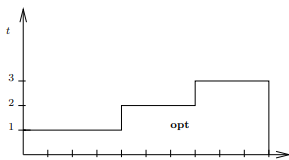
\includegraphics[]{chapters/introduction/histogram_opt.png}
        
        Now we construct another histogram for the greedy solution. We have $m$ columns, one for every set $S_i$. We order the columns (i.e sets) in the order they are covered by the greedy algorithm but the height of each column, rather than the timestep at which it was covered is now the price, as defined previously. The total area of the histogram is exactly equal to $\textbf{price}=\textbf{greedy}$. \\
        
        What we want to show is that $\textbf{price}$ is at most 4 times $\textbf{opt}$. The way we show that is by shrinking the second histogram by a factor of 4 and show that it fits completely inside the optimal histogram. The way we do that is by shrinking the height and the width by a factor of 2. Therefore, for each column we have a height of $p_i / 2$ and the width of the histogram is now $m/2$. \\
        
        Now, we align the greedy histogram to the right of the optimal histogram so that it occupies the space from $m/2 + 1$ up to $m$ on the horizontal axis. Now we claim that the shrunk greedy histogram is completely inside the optimal histogram and therefore this proves Lemma \ref{l:static_greedy}.
        
        \begin{figure}
            \centering
            \begin{subfigure}{.5\textwidth}
              \centering
              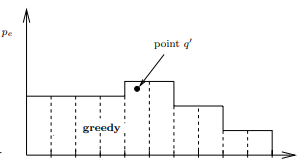
\includegraphics[width=.4\linewidth]{chapters/introduction/histogram_greedy.png}
              \caption{The greedy histogram before shrinking}
              \label{fig:sub1}
            \end{subfigure}%
            \begin{subfigure}{.5\textwidth}
              \centering
              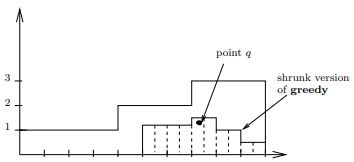
\includegraphics[width=.4\linewidth]{chapters/introduction/histogram_fit.png}
              \caption{Shrinking and Alignment}
              \label{fig:sub2}
            \end{subfigure}
            \label{fig:test}
        \end{figure}
        
        Consider an arbitrary point q' in the original (unshrunk) greedy histogram and let $S$ be the set it corresponds to. Let $i$ be the time step at which it was covered, then the height of this column is at most $\frac{|R_i|}{|X_i|}$ and the distance of q' from the right boundary of the optimal histogram is at most $R_i$. Now by shrinking we map the point q' to a new point q. The height of this point is now $h \leq \frac{|R_i|}{2 \cdot |X_i|}$ and the its distance from the right boundary is at most $r \leq \frac{|R_i|}{2}$. \\
        
        For our point q to lie within the optimal histogram it suffices to show that at timestep h at least r sets remain uncovered by the optimal algorithm. Consider the sets on $R_i$. No number can ever cover more than $|X_i|$ sets since our greedy algorithm selects at every time step the number that covers the most sets (and that is $|X_i$ at time step $i$). Therefore in $\floor{h}$ steps the optimal algorithm could cover at most $\floor{h} \cdot \floor{|X_i|} \leq \frac{|R_i|}{2}$ sets and therefore leave at least $|R_i| - \frac{|R_i|}{2} \geq \ceil{r}$ sets uncovered which proves our proposition that q lies within the optimal histogram.
    \end{proof}
    
    By the proof of Lemma \ref{l:static_greedy} we obtain that $\textbf{opt} \geq \textbf{price} / 4$ and since $\textbf{price} = \textbf{greedy}$ we have the proof of our original lemma.
    
\end{proof}

A natural question is whether the approximation ratio of this algorithm can be improved. To answer that we present the following hardness result.

\begin{theorem}\label{t:mssc_hardness}
    For every $\epsilon > 0$ it is NP-Hard to approximate min sum set cover within a ratio of $4-\epsilon$.
\end{theorem}

The authors of \cite{FLT04} continue by proving equivalent results for constrained versions of the problem as well as for the Min-Sum Vertex Cover, in which essentially every set $S_i$ has a cardinality of 2. Even though the algorithms they propose build an interesting intuition regarding the problem as we move on to generalized versions of the problem we observe that purely combinatorial tools are not sufficient to tackle the problem. This observation leads to the use of Linear Programming Relaxation methods which we use extensively while deriving our own results. To get a better idea of an Linear Programming approach we study a natural Generalization of the Min-Sum Set Cover problem \cite{SW11} and a randomized rounding schema that highlights several techniques. 